\chapter{Development of novel virtual-navigation decision-making behaviors} \label{chapter_2}

\section{Introduction}

In order to understand how cortical circuits perform the computations underlying decision-making, we must be able to record from and manipulate these circuits during decision tasks. We therefore need to develop well-characterized and controlled behaviors which enable us to accurately attribute changes in neuronal activity to specific features of the decision-making process. 

\bigskip
Here, we have developed three novel virtual reality (VR) decision tasks based on a T-maze. In the first task, mice are required to accumulate six discrete evidence cues to determine whether to turn into the left or right arm of the T-maze for a reward. In the second task, which has a delayed-match-to-sample design, mice are presented with only one cue, but the association between the cue and the turn direction can vary from trial to trial and is unknown to the mouse during cue presentation and during a delay period of several seconds. This task therefore allows for the dissociation of activity related to sensory information from that related to motor planning \citep{Freedman:2011hq}. The third and most difficult task incorporates components of both previous tasks to create an evidence accumulation task with a delayed-match-to-sample design.

\section{A virtual reality system for mouse behavior} \label{sec:vr}

To develop these behaviors, we have used a modified version of the previously developed VR system \citep{Harvey:2009ci,Harvey:2012du,Dombeck:2010jr}. In this system, head-restrained mice are surrounded by a large, half-cylindrical screen on which a first-person view of a virtual environment is presented (Figure \ref{fig:2_1}). By running on a spherical treadmill, mice can navigate through this environment, allowing them to perform behavioral tasks for a reward.

\begin{figure}

\includegraphics[width=\textwidth]{figures/fig_2_1.pdf}
\caption[Schematic of virtual reality behavior system.]{\textbf{Schematic of virtual reality behavior system.}
\label{fig:2_1}}
\end{figure}

\bigskip
The VR system has several key advantages. First and most importantly, the use of virtual environments enables the rapid prototyping of task designs, because virtual environments can easily be changed, even within a behavioral session. Second, the comparatively small amount of space required for VR system as well as relatively short training sessions (usually less than an hour) allow for the training of many mice in parallel. Third, because the contents environment are completely controlled by the experimenter, the only stimuli present in the virtual environment are those which are intentionally included. Finally, because mice are head-restrained during VR behaviors, this system can be paired with optical imaging \citep{Harvey:2012du, Dombeck:2010jr}, enabling the recording and manipulation of large populations of neurons during behavior, as well as whole-cell electrophysiology \citep{Harvey:2009ci, Domnisoru:2013jp}.

\subsection{Detailed description}

First-person images of the virtual environment were back-projected onto a half-cylindrical screen with a diameter of 24 inches and a depth of 12 inches using a PicoP microprojector (MicroVision Inc.). Images were transformed to account for the shape of the screen. The spherical treadmill was a custom 8-inch ball made of open-cell Styrofoam foam. The spherical treadmill was supported by air to allow free rotation. Movement of the spherical treadmill was recorded using an optical sensor (Logitech MX518) positioned beneath the ball. Forward/backward translation in VR was controlled by changes in pitch (relative to the mouse's body), and rotation in VR was controlled by changes in roll (relative to the mouse’s body). This is different from previous studies \citep{Harvey:2012du, Harvey:2009ci, Dombeck:2010jr}, in which rotation in VR was controlled by changes in yaw rather than roll (relative to the mouse’s body). This modification significantly improved the mouse's control of rotation in the virtual environment. The recorded behavioral parameters were the mouse’s position in the virtual environment (x/y position), the rotational velocity of the spherical treadmill (about the pitch and roll axes relative to the mouse’s body), and the mouse's view angle in the environment. Virtual environments were built and run using the MATLAB-based software ViRMEn (Virtual Reality Mouse Engine) \citep{Aronov:2014hn}. 

\section{Fixed association evidence accumulation task} \label{sec:fixed_section}

\subsection{Task description} \label{sec:fixed_task}

\begin{figure}

\includegraphics[width=\textwidth]{figures/fig_2_2.pdf}
\caption[A fixed association evidence accumulation task in virtual reality.]{\textbf{A fixed association evidence accumulation task in virtual reality. a,} Schematic of an example 2-4 right trial in a virtual T-maze. Asterisk marks the reward location. \textbf{b,} Sequence of trial events. \textbf{c,} Performance for five mice (mean $\pm$ s.e.m, 7-12 sessions).
\label{fig:2_2}}
\end{figure}

We developed a navigation-based evidence accumulation task for head-restrained mice based on a T-maze in VR (Figure \ref{fig:2_2}a-b). While running down the stem of the T with predominantly gray walls, mice encountered six visual cues (white wall segments with black dots) at fixed locations. Each cue could appear on either the left or right wall, and only one cue was visible at a time. Cue visibility was determined by the mouse’s position such that the duration of each cue was determined by the mouse’s running speed. On average, each cue was visible for $\sim$0.8 seconds. To receive a reward, mice had to determine if more cues were presented on the left or the right and, after a short stretch of maze without additional cues (90 cm, $\sim$1 second), turn at the T-intersection toward the direction that had more cues. Between trials, the task difficulty was modulated by varying the difference between the number of left and right cues, or the net evidence. Within each trial, there were six total cues, with between zero and six cues presented on the left and the remainder on the right. For example, a trial with six cues on the left and no cues on the right (6-0 left, net evidence: 6 left) was easy, while a trial with two cues on the left and four cues on the right (2-4 right, net evidence: 2 right) was much more difficult. The sequence of cues was determined randomly for each trial of a given net evidence. To perform well on this task, mice must accumulate multiple, discrete pieces of evidence across long timescales ($\sim$5-6 seconds) and remember their choice during a short delay ($\sim$1 second). By accumulating multiple pieces of evidence, mice were able to perform this task at high accuracy stably for many days (Figure \ref{fig:2_2}c).

\subsection{Training procedure} \label{sec:fixed_train}

\begin{figure}
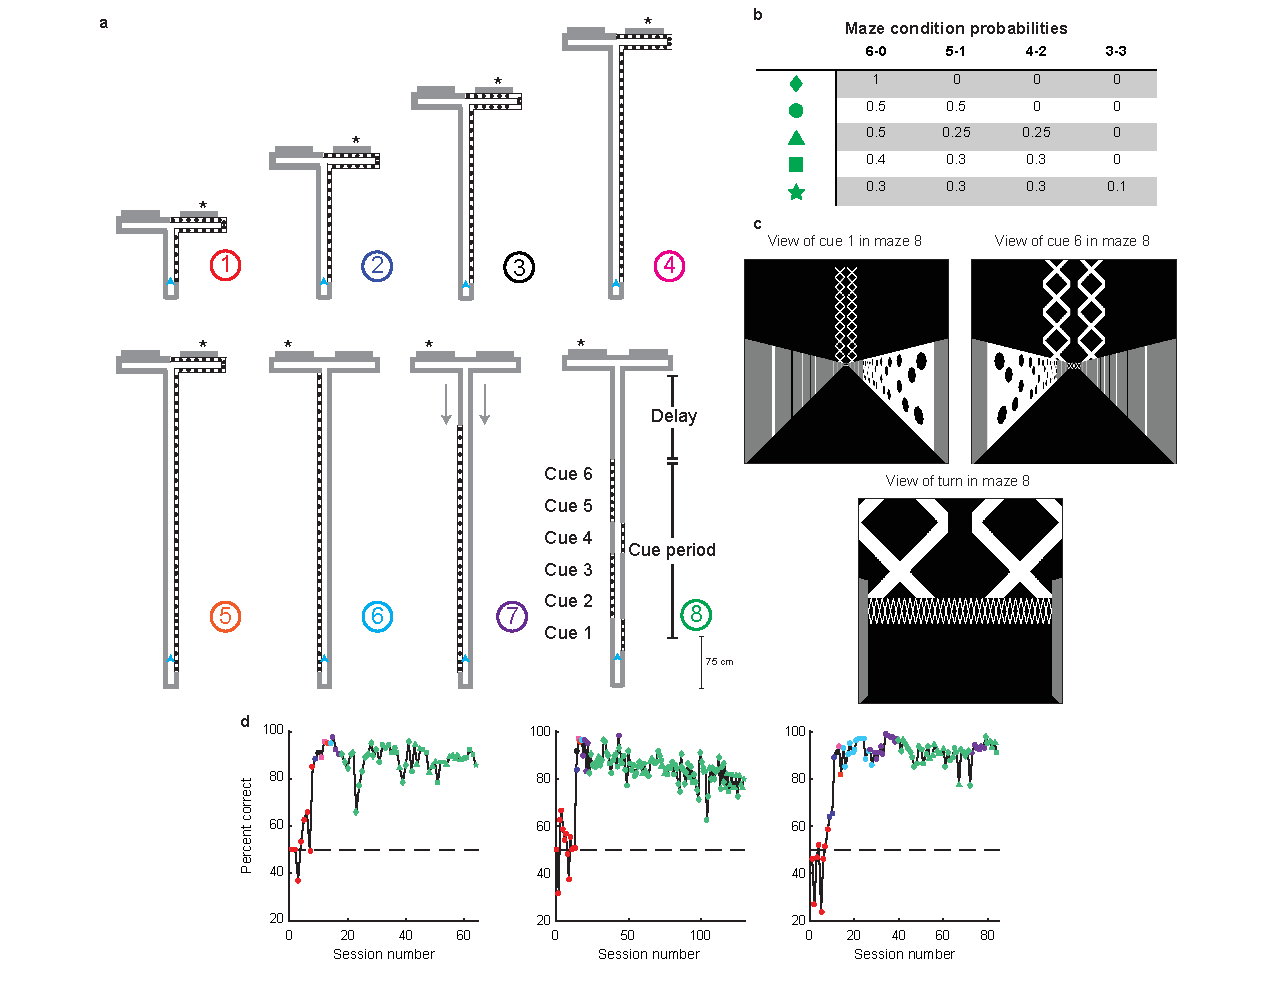
\includegraphics[width=\textwidth]{figures/fig_2_3.pdf}
\caption[Behavioral training procedure for the fixed association evidence accumulation task]{\textbf{Behavioral training procedure for the fixed association evidence accumulation task. a,}
Sequence of mazes used for behavioral training. Asterisks indicate reward location. Only some example mazes are shown (for example, right choice and not left choice maze in maze 1). 
%
\textbf{b,} Distribution of net evidence corresponding to different difficulties used in training the final task (maze 8; see \textbf{d}). 
%
\textbf{c,} Screen captures of the virtual environment at cue 1, cue 6, and the turn in maze 8. 
%
\textbf{d,} Behavioral performance across sessions for three example mice. Colors correspond to the maze colors indicated in \textbf{a}. Shapes correspond to the net evidence probabilities in \textbf{b}.
\label{fig:2_3}}
\end{figure}

Following at least two days of water restriction, mice began behavioral training. Behavioral sessions were performed six days per week and lasted 45-60 minutes. Mice received liquid rewards through a lick spout (4\textmu l/reward, 10\% sweetened condensed milk). Mice were trained to perform the evidence accumulation task over a series of eight mazes (Figure \ref{fig:2_3}). In mazes 1-5, mice learned to steer in the virtual environment and to associate visual cues with a reward. In mazes 6-7, mice learned to remember the location of the cue during a brief delay period ($\sim$1 second). In maze 8, the initially continuous white cue on either the left or the right was divided into 6 discrete cues, all of which were on the same side (e.g. 6-0 left and 0-6 right trials). Cue visibility was locked to the mouse’s position such that only one cue was visible at a time. There was no delay between the offset of one cue and the onset of the next cue. At this point, the probability of more difficult conditions (e.g. 5-1 trials) was gradually increased using the probability distributions in Figure \ref{fig:2_3}b. Within each difficulty, the precise pattern of evidence was randomly determined before each trial. On 3-3 trials, the rewarded location was selected randomly. Trials were completed when the mouse turned into one of the arms of the T-maze. Following the completion of the trial, the screen changed to black for the duration of the inter-trial interval (ITI; 2 s for correct choice and 4 s for incorrect choice).
 
\bigskip
In some cases, mice developed biases such that they favored left or right choices. To discourage these biases, we implemented bias correction throughout training. Bias correction was not used during the imaging sessions described in Chapter \ref{chapter_3}. On each trial, we determined a probability that a trial would be a right choice trial. The probability was set to be equal to the fraction of left choices over the previous 20 trials, such that if the mouse had made many left or right choices previously then the opposite choice trial was likely selected. Once mice reached expert levels, prolonged biases rarely developed. To maintain a high level of performance throughout the session, we introduced a small fraction of easy trials (‘crutch trials’) interleaved with the evidence accumulation trials. Crutch trials were identical to trials from maze 5 (Figure \ref{fig:2_3}) in which no evidence accumulation or delay were present. The probability of a crutch trial on a given trial was equal to the fraction of error trials over the previous 20 trials. We found that the use of crutch trials was essential to establishing stable behavior both within a single session and across multiple sessions.

\bigskip
For mazes 1-3, the criterion for advancement to the next maze was the mouse’s number of completed trials per minute, independent of performance (> 7 trials/min for advancement). Mice on mazes 4-5 were advanced to the next maze following one day of ≥ 90\% performance. Mice on mazes 6-7 were advanced following three days of ≥ 90\% performance. On maze 8, mice were advanced after three days of ≥ 85\% performance on easy trials (6-0 and 5-1 trials) and ≥ 65\% performance on hard trials (4-2 trials). At this stage of training, mice were sensitive to the rapid introduction of difficult trials, and performance on easy trials was closely monitored. If performance on easy trials fell below 80\%, mice were moved to an easier distribution of maze trials. For this reason, we were only able to introduce 3-3 trials in some of the mice. Training in total required $\sim$30-60 daily training sessions (Figure \ref{fig:2_3}d). 

\subsection{Behavioral characterization} \label{sec:fixed_behav}

\begin{figure}
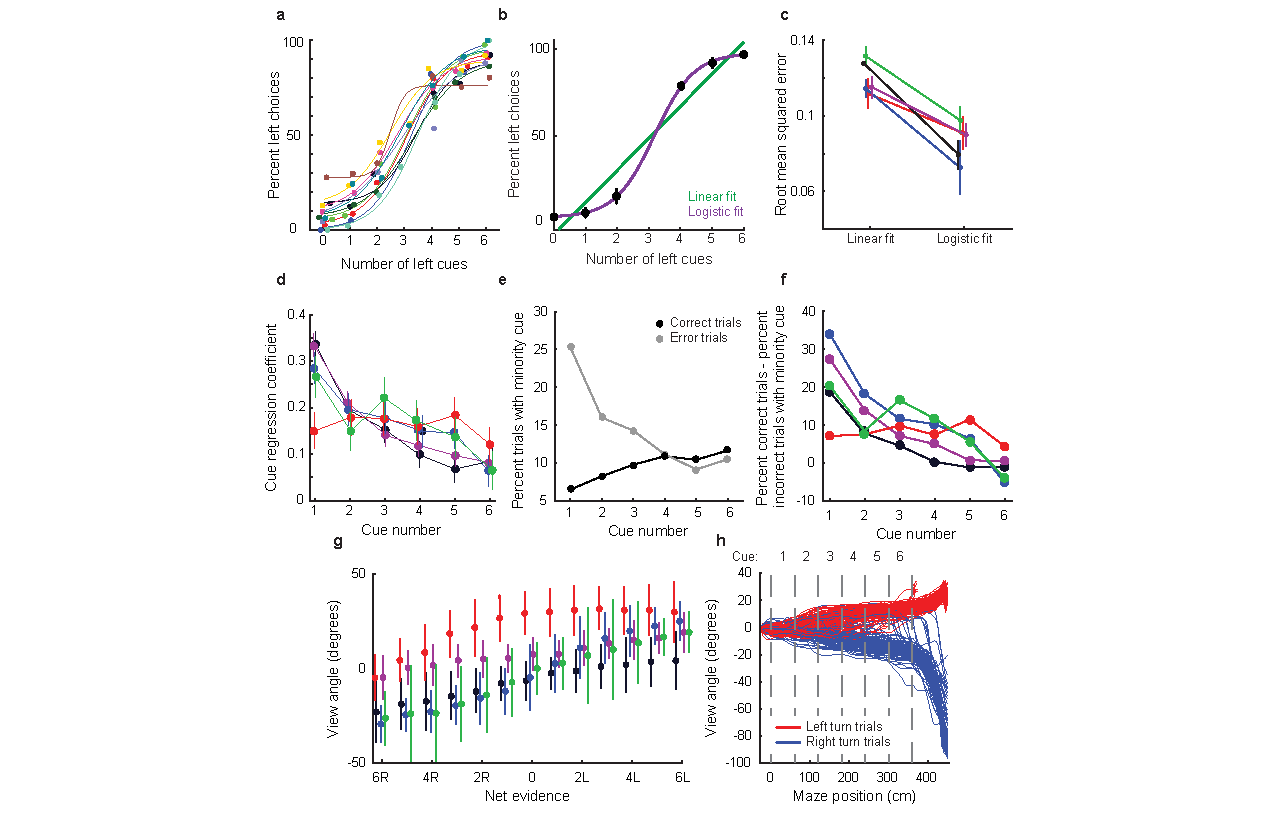
\includegraphics[width=1.5\textwidth,center]{figures/fig_2_4.pdf}
\caption[Behavioral characterization of the fixed association evidence accumulation task.]{
\textbf{Behavioral characterization of the fixed association evidence accumulation task. a,} Psychometric functions describing behavioral performance on individual behavioral sessions. Each of these sessions was used to acquire imaging data in Chapter \ref{chapter_3} Data were fit with a logistic function. 
%
\textbf{b,} Example performance from a single mouse across seven behavioral sessions fit by a linear (green) and logistic (purple) model. 
%
\textbf{c,} Across mice, the logistic model fit the data significantly better than the linear model (p < 0.05 for all mice, two-sample Student's t-test), suggesting that mice used more than one piece of evidence per trial to make a choice. Error bars represent mean $\pm$ s.e.m. across datasets. Mice are colored the same as in Figure \ref{fig:2_2}c.
%
\textbf{d,} Multivariate linear regression in which the mouse's choice was the response variable and the six cue identities were separate explanatory variables. Regression coefficients for five mice (7-12 sessions each) are shown. Four of the five mice weighted early cues more than late cues. Error bars indicate confidence intervals. Mice are colored the same as in Figure \ref{fig:2_2}c.
%
\textbf{e-f,} Fraction of correct (black) and error (gray) trials containing a minority cue (a cue indicating the incorrect choice) at each cue position, for a single mouse (\textbf{e}) and as the difference of the error and correct points (\textbf{f}) for five mice. Mice are colored the same as in Figure \ref{fig:2_2}c. 
%
\textbf{g,} Relationship between net evidence and view angle for each mouse combined across all cue positions. Mice are colored the same as in Figure \ref{fig:2_2}c.
%
\textbf{h,} View angle as a function of maze position for individual trials within an example session. Traces are colored according to whether the mouse turned left (red) or right (blue).
\label{fig:2_4}}
\end{figure}


Mice could have achieved intermediate performance on this task by only paying attention to a single cue. A mouse perfectly following this strategy would be expected to make a correct choice on 100\% of 6-0 trials (because every cue matches the correct choice), 83\% on 5-1 trials (because each cue has a 5/6 chance of matching the correct choice), and 67\% on 4-2 trials. The psychometric functions of each mouse would therefore be approximately linear. If, however, mice used more than one cue to make their decisions, their psychometric functions should look approximately sigmoidal. We therefore fit the behavioral performance as a function of number of left cues with a logistic function (assuming more than one piece of evidence used per trial) and a linear function (assuming a single piece of evidence used per trials) using maximum-likelihood estimation. To compare linear and logistic model fits each behavioral day of each mouse was fit separately by both models, and the distribution of root mean squared errors (RMSE) was compared with a two-sample Student’s t-test. Across mice, the logistic function fit the data significantly better than the linear function (Figure \ref{fig:2_4}a-b), indicating that mice used more than one piece of evidence per trial. It is worth noting that this analysis does not demonstrate that mice used all six cues; it only shows that mice used more than one. Unfortunately, the precise analysis of each mouse's strategy was not possible due to limited trial numbers, especially on trials with ambiguous evidence.

\bigskip
Because mice did not perform the task optimally, it is possible that they weighted some evidence cues more than others. To test if cues were weighted equally, we used multivariate linear regression, with the behavioral choice as the dependent variable and the cue identities as the explanatory variables. To include large numbers of trials, multiple consecutive sessions (mean: 9, range: 7-12) were combined. We found that all cues had significant regression coefficients with a preference toward earlier segments, suggesting that mice accumulated evidence with a primacy bias (Figure \ref{fig:2_4}d). To confirm this result, we performed a complementary analysis in which we analyzed the location of minority cues (cues indicating the incorrect choice) on correct and error trials. We found that minority cues were uniformly distributed on correct trials, but more likely to appear in early cue positions on error trials (Figure \ref{fig:2_4}e-f). This results suggests that mice were more likely to make an error when a minority cue was present as one of the first cues.  Mice exhibit a primacy bias even though the optimal strategy for this task is to take into account all six cues (as long as at least one trial is present in which the sixth cue provides information). This suggests that mice must have placed some weight on making decisions early, before all six cues had been presented. Interestingly, this unequal weighting of cues was not present in all mice, as one mouse (colored in red in Figures \ref{fig:2_2} and \ref{fig:2_4}) weighted all cues approximately equally. 

\bigskip
We also found there to be a notable correlation between the net accumulated evidence and the mouse’s view angle (Figure \ref{fig:2_4}g). As a result, the view angles of left and right turn trials diverged well before the end of the cue period (Figure \ref{fig:2_4}h). This correlation highlights one of the downsides of closed-loop tasks in which the association between sensory cues and choices is fixed: animals may change their behavior, and hence, the features of the sensory cues in response to prior sensory cues, introducing undesirable correlations between sensory and motor variables. These correlations can make the precise interpretation of neural responses challenging. As discussed in more detail in Chapter \ref{chapter_3}, we were therefore careful to ensure that neural results could not be wholly explained by these differences in behavior. 

\bigskip
To test whether there was a relationship between the mouse’s choice on a trial and the outcome of the previous trial, we used a multivariate logistic regression with interactions with the previous trial’s choice and reward outcome (whether the previous trial was correct or incorrect) as binary explanatory variables and the mouse’s choice on the test trial as the response variable. We combined multiple consecutive sessions (mean: 9, range: 7-12) to include large numbers of trials. Consistently, this model was unable to predict the mouse’s choice, suggesting that there was no easily detectable behavioral relationship between the mouse’s choice and the outcome of the previous trial (R\textsuperscript{2}: 0.02 $\pm$ 0.01, mean $\pm$ s.e.m across datasets, p > 0.05). 

\section{Delayed-match-to-sample task} \label{sec:dms}

\subsection{Task description}

\begin{figure}
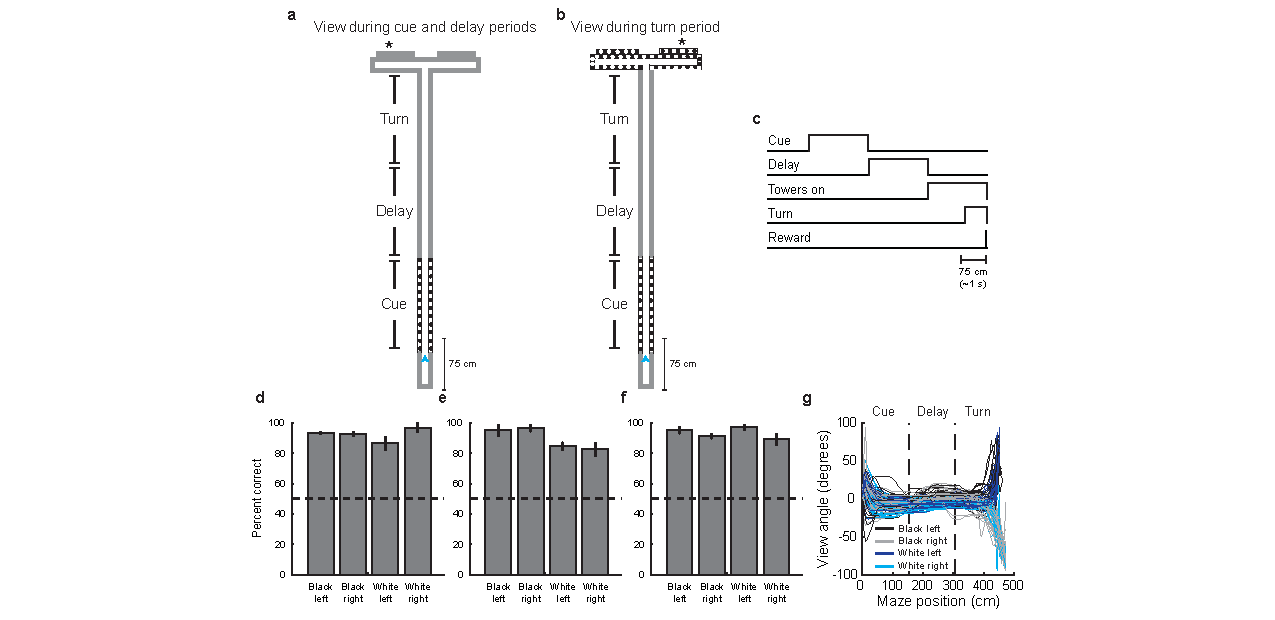
\includegraphics[width=1.4\textwidth,center]{figures/fig_2_5.pdf}
\caption[A delayed-match-to-sample task in virtual reality.]{\textbf{A delayed-match-to-sample task in virtual reality. a-b,} Schematic of an example white cue trial during the cue or delay period (\textbf{a}) and during the turn period (\textbf{b}). Asterisk marks the reward location.
%
\textbf{c,} Sequence of trial events. 
%
\textbf{d-f,} Performance for three example mice broken up by trial configuration (mean $\pm$ s.e.m, 4-8 sessions).
%
\textbf{g,} View angle as a function of maze position for individual trials within an example session. Traces are colored according to trial configuration. Note that traces do not separate according to choice until the turn period and that there is a systematic difference between black and white trials during the delay period.
\label{fig:2_5}}
\end{figure}

This task is a navigation-based decision task with a non-fixed association between sensory evidence and choice. As with the fixed association task described above, this task is designed for head-restrained mice and is based on a T-maze in VR with two towers positioned behind the arms of the T (Figure \ref{fig:2_5}a-c). During the cue period at the beginning of the trial, mice encounter an extended stretch of wall which is either predominantly black or white with dots of the opposite color. As mice run down the stem of the T, they enter a several second delay period in which the walls are gray, independent of the cue identity. During both the cue and delay periods, the arms and towers at the end of the T-maze are gray. At the conclusion of the delay period, the coloring of one of the arms (along with its corresponding tower) changes to white with black dots while the other changes to black with white dots. To receive a reward, the mouse must turn toward the arm which matches the cue presented during the cue period. There are therefore four trial configurations (two cues combined with two turns). Critically, the association between the cue and the rewarded turn is variable from trial to trial, such that during the cue and delay periods, the mouse does not know which direction it will need to turn for a reward. Thus, mice must remember the cue during the delay period, abstracted from a motor plan. The delayed-match-to-sample design of this task therefore allows the separation of neuronal signals related to the memory of sensory cue from those related to a motor plan \citep{Freedman:2011hq}.

\bigskip
Mice were able to perform this task successfully across all four trial configurations (e.g., a black cue with a rewarded left turn; Figure \ref{fig:2_5}d-f). The consistent performance across trial conditions suggests that mice were not significantly biased. For example, if mice exhibited a bias toward left choices, performance would be high on conditions in which left choices are rewarded (i.e., black left and white left) and low on conditions in which right choices are rewarded (i.e., black right and white right). Alternatively, mice may have exhibited a cue-specific bias, in which they are more likely to turn left on black cue trials and right on white cue trials. This type of bias would result in high performance on those trials, but low performance on opposite turn trials. While weak versions of these biases appeared (for example, the mouse displayed in Figure \ref{fig:2_5}f had a weak left choice bias), these biases were not significant. Interestingly, mice often performed well on three out of the four conditions, suggesting that mice did not learn an abstract rule to match the cue presented during the cue period to the arms, but instead memorized configurations (e.g., when the cue is white and white is on the left, go left).

\subsection{Training procedure} \label{sec:dms_train}

\begin{figure}
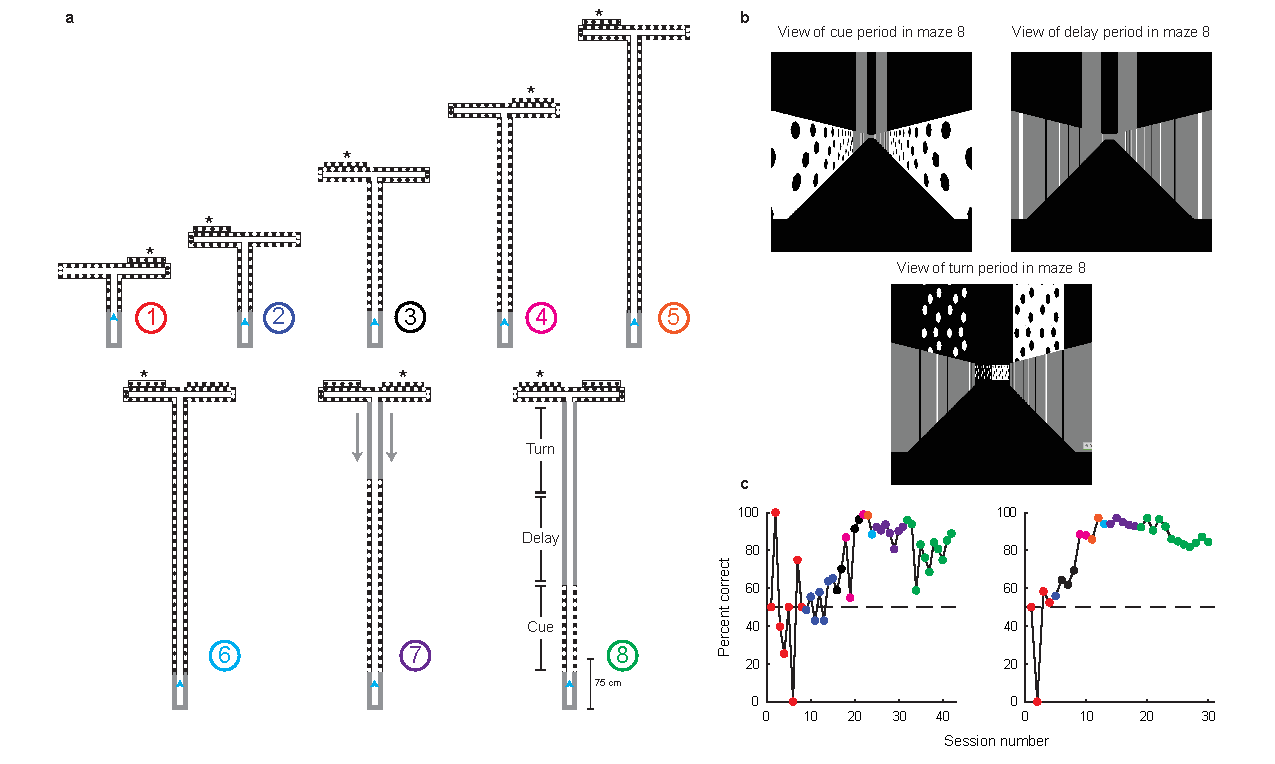
\includegraphics[width=1.05\textwidth,center]{figures/fig_2_6.pdf}
\caption[Behavioral training procedure for the delayed-match-to-sample task]{\textbf{Behavioral training procedure for the delayed-match-to-sample task. a,}
Sequence of mazes used for behavioral training. Asterisks indicate reward location. Only some example mazes are shown (for example, white right maze in maze 1).  
%
\textbf{b,} Screen captures of the virtual environment during the cue, delay and turn periods in maze 8. 
%
\textbf{c,} Behavioral performance across sessions for two example mice. Colors correspond to the maze colors indicated in \textbf{a}. 
\label{fig:2_6}}
\end{figure}

Following at least two days of water restriction, mice began behavioral training. Behavioral sessions were performed six days per week and lasted 45-60 minutes. Mice received liquid rewards through a lick spout (4\textmu l/reward, 10\% sweetened condensed milk). Mice were trained to perform the delayed-match-to-sample task over a series of eight mazes (Figure \ref{fig:2_6}). In mazes 1-5, mice progressed through a series of mazes of increasing length which taught them to steer in the virtual environment and to associate visual cues with a reward. This progression is similar to that used in the training for the fixed association evidence accumulation task, but the mazes used to train the delayed-match-to-sample task were structured slightly differently. In each of these mazes, both walls of the stem contained either the white or black cue and the arms contained both cues, with one on the left and one on the right. The correct arm, which matched the cue present in the stem of the maze, was indicated by a tower colored with the same cue which was located behind the rewarded arm. The unrewarded arm did not have a tower behind it. Mice could therefore achieve perfect performance on these mazes by turning toward the arm with a tower without paying attention to the cues on the walls of the T-maze. The trial configuration was randomly selected from the four possibilities prior to each trial. Importantly, all four configurations were present during these early mazes to prevent mice from learning a spurious association between a cue and a choice (e.g., turn left when a black cue is present).

\bigskip
In maze 6, an additional tower was added behind the unrewarded arm as well, forcing mice perform a non-delayed-match-to-sample in which they must turn toward the arm whose coloring matches the cue presented in the stem of the maze. When we first attempted this transition, mice were unable to learn it, rapidly dropping to chance performance and picking up strong biases (e.g., always turn left). To ease mice into this transition, consecutive trials were ‘paired’, such that a trial with a single tower (as in maze 5) always preceded a trial with two towers (as in maze 6). Critically, these paired trials had the same configuration and mice received three times as many rewards for making a correct choice on the two tower trial. Because consecutive trials featured the same reward location in this paired organization, this structure may have taught mice to repeat a rewarded choice. However, we found that mice rarely learned this strategy, and that the paired organization helped mice to rapidly achieve high performance on maze 6, often within a single day (see cyan points in Figure \ref{fig:2_6}c). 

\bigskip
Maze 7 begins identically to maze 6, except visibility of the arm configuration is obscured until mice pass the 2/3 point of the stem. However, because there is no delay period yet, this maze still only requires a non-delayed-match-to-sample. As mice performed trials correctly, a delay (in the form of gray walls separating the cue and arms) would slowly appear, increasing in length as mice performed more and more trials correctly. Once the length of the delay reached 1/3 of the stem, mice performed an instantaneous-match-to-sample, in which the cue and arm configuration were no longer visible simultaneously. As the delay length increased beyond this point, mice performed a delayed-match-to-sample task with an increasingly longer delay period. Maze 8 appeared identically to the final version of maze 7, in which the cue, delay, and turn periods each extended for 1/3 of the maze stem.

\bigskip
As with the fixed association task, bias correction was introduced beginning with maze 4. Bias correction was applied to both turn direction and arm configuration independently. Prior to each trial, the probability that a left choice would be rewarded was set to the fraction of right choices over the preceding 20 trials. The probability that a turn towards a white arm would be rewarded was set to the fraction of turns toward black arms over the preceding 20 trials. For example, if a mouse turned left 75\% of the time and toward black arms 75\% of the time, then the probability of the next trial being black left would be 0.0625 (0.25 $\times$ 0.25), being black right 0.1875 (0.25 $\times$ 0.75), being white left 0.1875 (0.75 $\times$ 0.25) and being white right 0.5625 (0.75 $\times$ 0.75). Crutch trials were introduced as well, beginning with maze 7. Crutch trials were identical to trials from maze 6 (Figure \ref{fig:2_6}a). As with the fixed association task, the probability of a crutch trial was set to the fraction of error trials over the preceding 20 trials. 

\bigskip
For mazes 1-3, the criterion for advancement to the next maze was the mouse’s number of completed trials per minute, independent of performance (> 7 trials/min for advancement). Mice on mazes 4-5 were advanced to the next maze following one day of ≥ 90\% performance. Mice on maze 6 were advanced following one day of ≥ 80\% performance on trials with two towers. In maze 7, delay advancement was controlled according to the following rule. After the first 30 trials of a session, the delay advanced by 1/60 of the stem whenever mice performed three consecutive correct trials. Advancement was halted for at least 30 trials every 1/6 of the maze, creating a block structure of advancement (e.g., once the delay had reached 1/6 of the stem, 2/6 of the stem, etc.). To resume delay advancement, mice must have performed 75\% of the preceding 30 trials correctly. On consecutive training sessions, mice were reset to the last block on which they had high accuracy. For example, if a mouse ended a session with a delay of 27/60, the next session would begin with a delay of 2/6. This process continued until mice had accuracy ≥ 75\% on sessions beginning with a delay of 2/3, at which point they were advanced to maze 8. Training in total required $\sim$20-40 daily training sessions (Figure \ref{fig:2_3}d). This task was difficult to train; only about one-quarter of the mice who begin training eventually reached high accuracy on the final task. 

\subsection{Behavioral characterization} \label{sec:dms_behav}

In contrast to the fixed association evidence accumulation task, mice did not demonstrate a strong association between view angle and choice during the cue and delay periods (Figure \ref{fig:2_5}g). This serves as a confirmation of the delayed-match-to-sample design of this task, as the mouse cannot know its choice until the turn period when the arm configuration is revealed (presuming the mouse is performing the task at high accuracy). Interestingly, there was a weak, but noticeable, relationship between the cue and the mouse’s view angle during the delay period. For example, the example mouse in Figure \ref{fig:2_5}g systematically turned toward the left during the delay period when it had seen a black cue and toward the right when it had seen a white cue. This effect suggests that mice may have used their view angle to remember the cue throughout the delay period, potentially complicating the interpretation of neuronal activity during the delay period, and removing some of the advantages of a delayed-match-to-sample task design. 

\bigskip
To test whether there was a relationship between the mouse’s choice on a trial and the outcome of the previous trial, we used the same multivariate logistic regression as we did for the fixed association evidence accumulation task. Consistent with that result, the model was unable to predict the mouse’s choice, again suggesting that there was no clear relationship between the mouse’s choice on trial \textit{n} and its choice on trial \textit{n+1} (R\textsuperscript{2}: 0.01 $\pm$ 0.01, mean $\pm$ s.e.m across datasets, p > 0.05). 

\section{Delayed-match-to-sample evidence accumulation task}

\subsection{Task description}

\begin{figure}
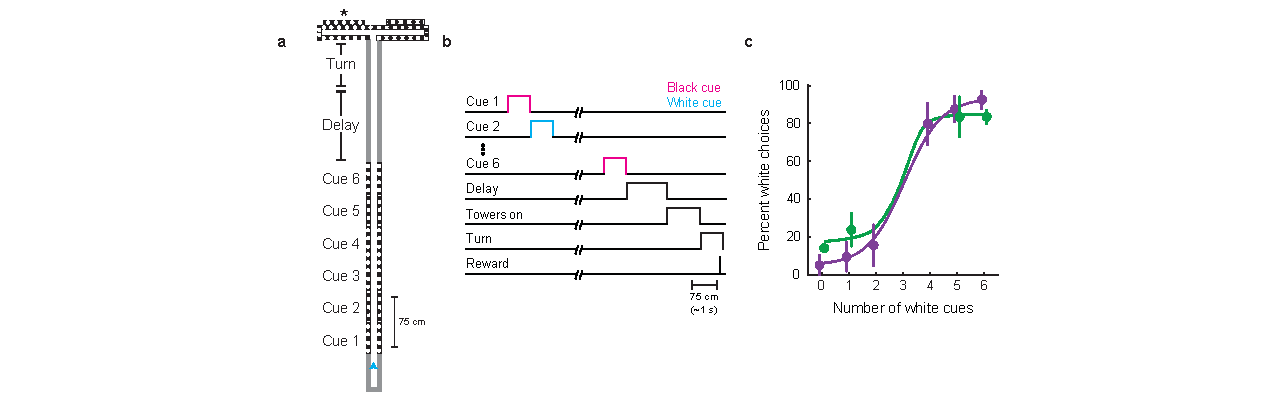
\includegraphics[width=1.4\textwidth,center]{figures/fig_2_7.pdf}
\caption[A delayed-match-to-sample evidence accumulation task in virtual reality.]{\textbf{A delayed-match-to-sample evidence accumulation task in virtual reality. a-b,} Schematic of an example 4-2 trial. Asterisk marks the reward location.
%
\textbf{b,} Sequence of trial events. 
%
\textbf{c,} Performance for two mice (mean $\pm$ s.e.m, 3 and 12 sessions for the green and purple mice, respectively).
\label{fig:2_7}}
\end{figure}

This task adds an evidence accumulation component to the delayed-match-to-sample task (Figure \ref{fig:2_7}a-b). As in the fixed association evidence accumulation task, as mice run down the stem of a T-maze, they are presented with six, discrete visual cues. In contrast to the fixed association task, these cues appear on both walls of the T-maze and can either be black or white (with dots of the opposite color). As in the delayed-match-to-sample task, the arm configuration is obscured (colored gray) until the conclusion of the delay period, at which point it becomes visible. To perform this task well, mice must decide whether there are more black or white cues, remember the accumulated cue identity throughout the delay, and then use the memory of the accumulated cue to make a choice toward the corresponding arm during the turn period. As in the delayed-match-to-sample task, mice cannot know which choice will be rewarded until the end of the delay period. Mice must therefore maintain a memory of the accumulated cue that is independent of the eventual motor choice throughout the cue and delay periods. 

\bigskip
This task is extremely difficult and inefficient to train; only four out of close to one hundred mice ever reached high accuracies on the final task, and of those, the performance of all but one was unstable from day to day. However, several mice were able to perform this task with high accuracy (Figure \ref{fig:2_7}c).    

\begin{figure}
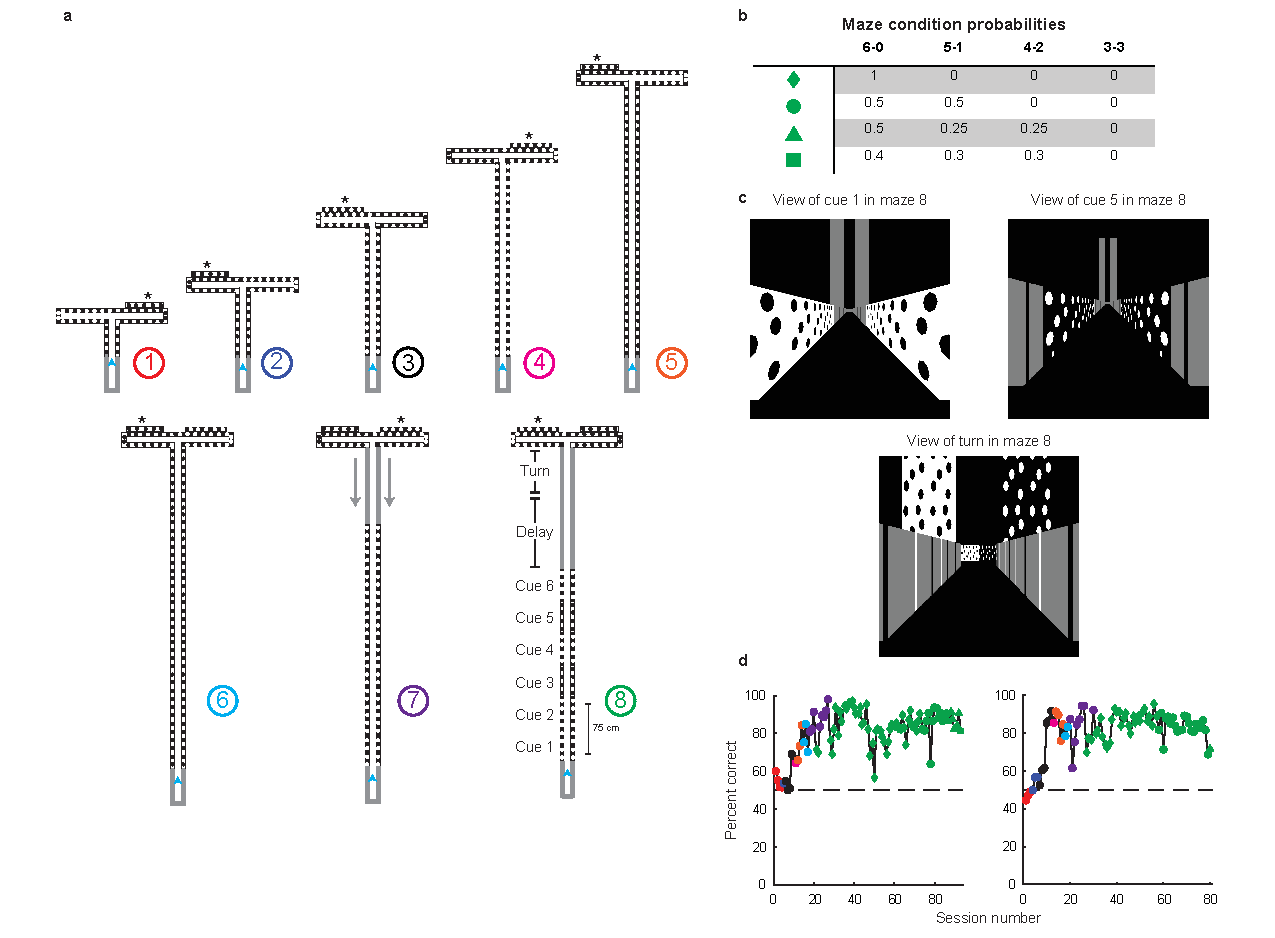
\includegraphics[width=\textwidth]{figures/fig_2_8.pdf}
\caption[Behavioral training procedure for the delayed-match-to-sample evidence accumulation task]{\textbf{Behavioral training procedure for the delayed-match-to-sample evidence accumulation task. a,}
Sequence of mazes used for behavioral training. Asterisks indicate reward location. Only some example mazes are shown (for example, white right maze in maze 1). 
%
\textbf{b,} Distribution of net evidence corresponding to different difficulties used in training the final task (maze 8; see \textbf{d}). 
%
\textbf{c,} Screen captures of the virtual environment at cue 1, cue 5, and the turn in maze 8. 
%
\textbf{d,} Behavioral performance across sessions for two example mice. Colors correspond to the maze colors indicated in \textbf{a}. Shapes correspond to the net evidence probabilities in \textbf{b}.
\label{fig:2_8}}
\end{figure}

\subsection{Training procedure} \label{sec:dms_int_train}

The first portion of training for this task was almost identical to the training for the delayed-match-to-sample task described in section \ref{sec:dms_train}. The only difference is that the cue period was lengthened to allow for the eventual discretization into six cues. Once mice performed the delayed-match-to-sample task stably across days with high accuracy, the cue period was divided into six discrete cues (maze 8). As with the fixed association evidence accumulation task, cue visibility was locked to the mouse’s position such that only one cue was visible at a time and there was no delay between the offset of one cue and the onset of the next cue. Initially, only 6-0 trials (trials in which all six cues were black or white) were included. More difficult conditions (5-1 and 4-2 trials) were gradually introduced according to the probability distributions in Figure \ref{fig:2_8}b. Only one mouse was ever able to successfully perform 4-2 trials and no mice were ever able to perform 3-3 trials without performance dropping significantly on easier trial conditions. Bias correction and crutch trials were included as in the training for the delayed-match-to-sample task. Training in total required $\sim$60-90 sessions. 

\subsection{Behavioral characterization} \label{sec:dms_int_behav}

As in the fixed association evidence accumulation task, we tested whether mice weighted some evidence cues more than others (Section \ref{sec:fixed_behav}). In contrast to the primacy bias observed in the fixed association task, a multivariate linear regression demonstrated that mice weighted cues approximately equally (Figure 2.9a). The analysis of minority cue location, however, suggested that mice had a noticeable recency bias, as minority cues were most likely to induce an error when they were located at the fifth and sixth cue positions (Figure 2.9b-c). 


\begin{figure}
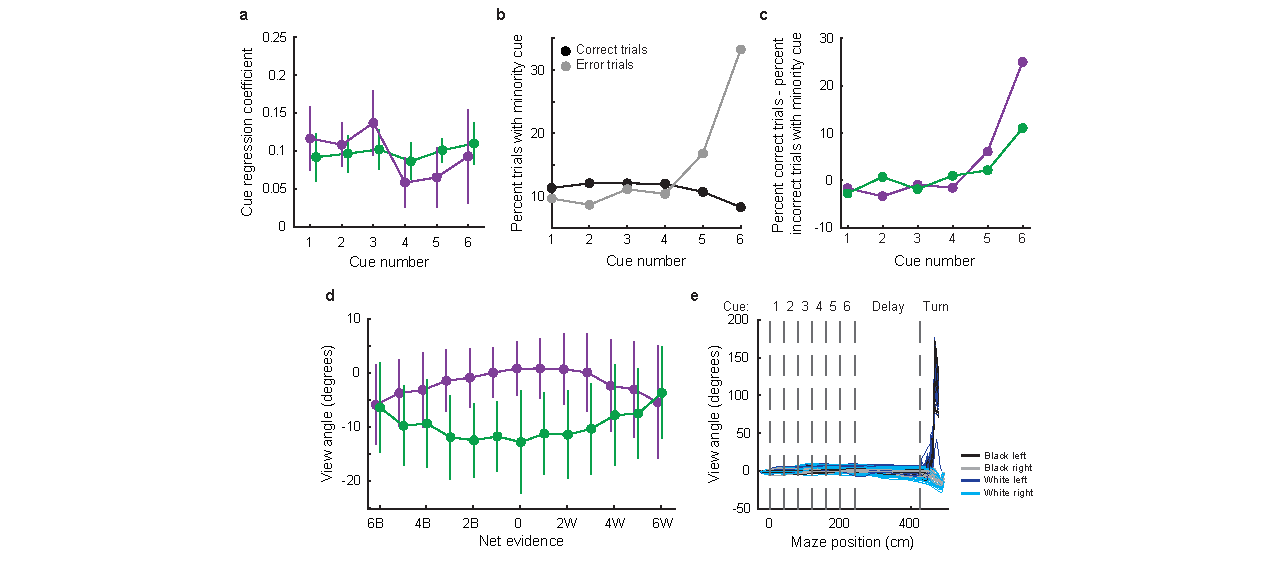
\includegraphics[width=1.4\textwidth,center]{figures/fig_2_9.pdf}
\caption[Behavioral characterization of the delayed-match-to-sample evidence accumulation task.]{
\textbf{Behavioral characterization of the delayed-match-to-sample evidence accumulation task. a,} Multivariate linear regression in which the mouse's choice was the response variable and the six cue identities were separate explanatory variables. Regression coefficients for two mice (3 and 12 sessions for the green and purple mice, respectively) are shown. Error bars indicate confidence intervals. Mice are colored the same as in Figure \ref{fig:2_7}c.
%
\textbf{b-c,} Fraction of correct (black) and error (gray) trials containing a minority cue (a cue indicating the incorrect choice) at each cue position, for a single mouse (\textbf{b}; mouse colored purple in \textbf{a, c, d}) and as the difference of the error and correct points (\textbf{c}) for both mice. Mice are colored the same as in Figure \ref{fig:2_7}c. 
%
\textbf{d,} Relationship between net evidence and view angle for each mouse combined across all cue positions. Mice are colored the same as in Figure \ref{fig:2_7}c.
%
\textbf{e,} View angle as a function of maze position for individual trials within an example session. Traces are colored according to the trial configuration.
\label{fig:2_9}}
\end{figure}

\bigskip
We also found there to be no systematic correlation between the net accumulated evidence and the mouse’s view angle (Figure 2.9d). As in the delayed-match-to-sample task, the mouse’s view angle was also unable to predict the mouse’s choice until the turn period (Figure 2.9e). Interestingly, the difference in view angle due to cue during the delay period that we observed during the delayed-match-to-sample task (see Section \ref{sec:dms_behav}) was absent during this task.

\bigskip
Finally, to test whether there was a relationship between the mouse’s choice on a trial and the outcome of the previous trial, we used the same multivariate logistic regression as we did for both previous tasks (Sections \ref{sec:fixed_behav} and \ref{sec:dms_behav}). Consistent with those results, the model was unable to predict the mouse’s choice, again suggesting that there was no clear relationship between the mouse’s choice on trial \textit{n} and its choice on trial \textit{n+1} (R\textsuperscript{2}: 0.01 ± 0.01, mean $\pm$ s.e.m across sessions for purple mouse, p > 0.05; 0.02 $\pm$ 0.01, mean ± s.e.m across sessions for green mouse, p > 0.05). 

\section{Behavioral analysis suite}

\begin{figure}
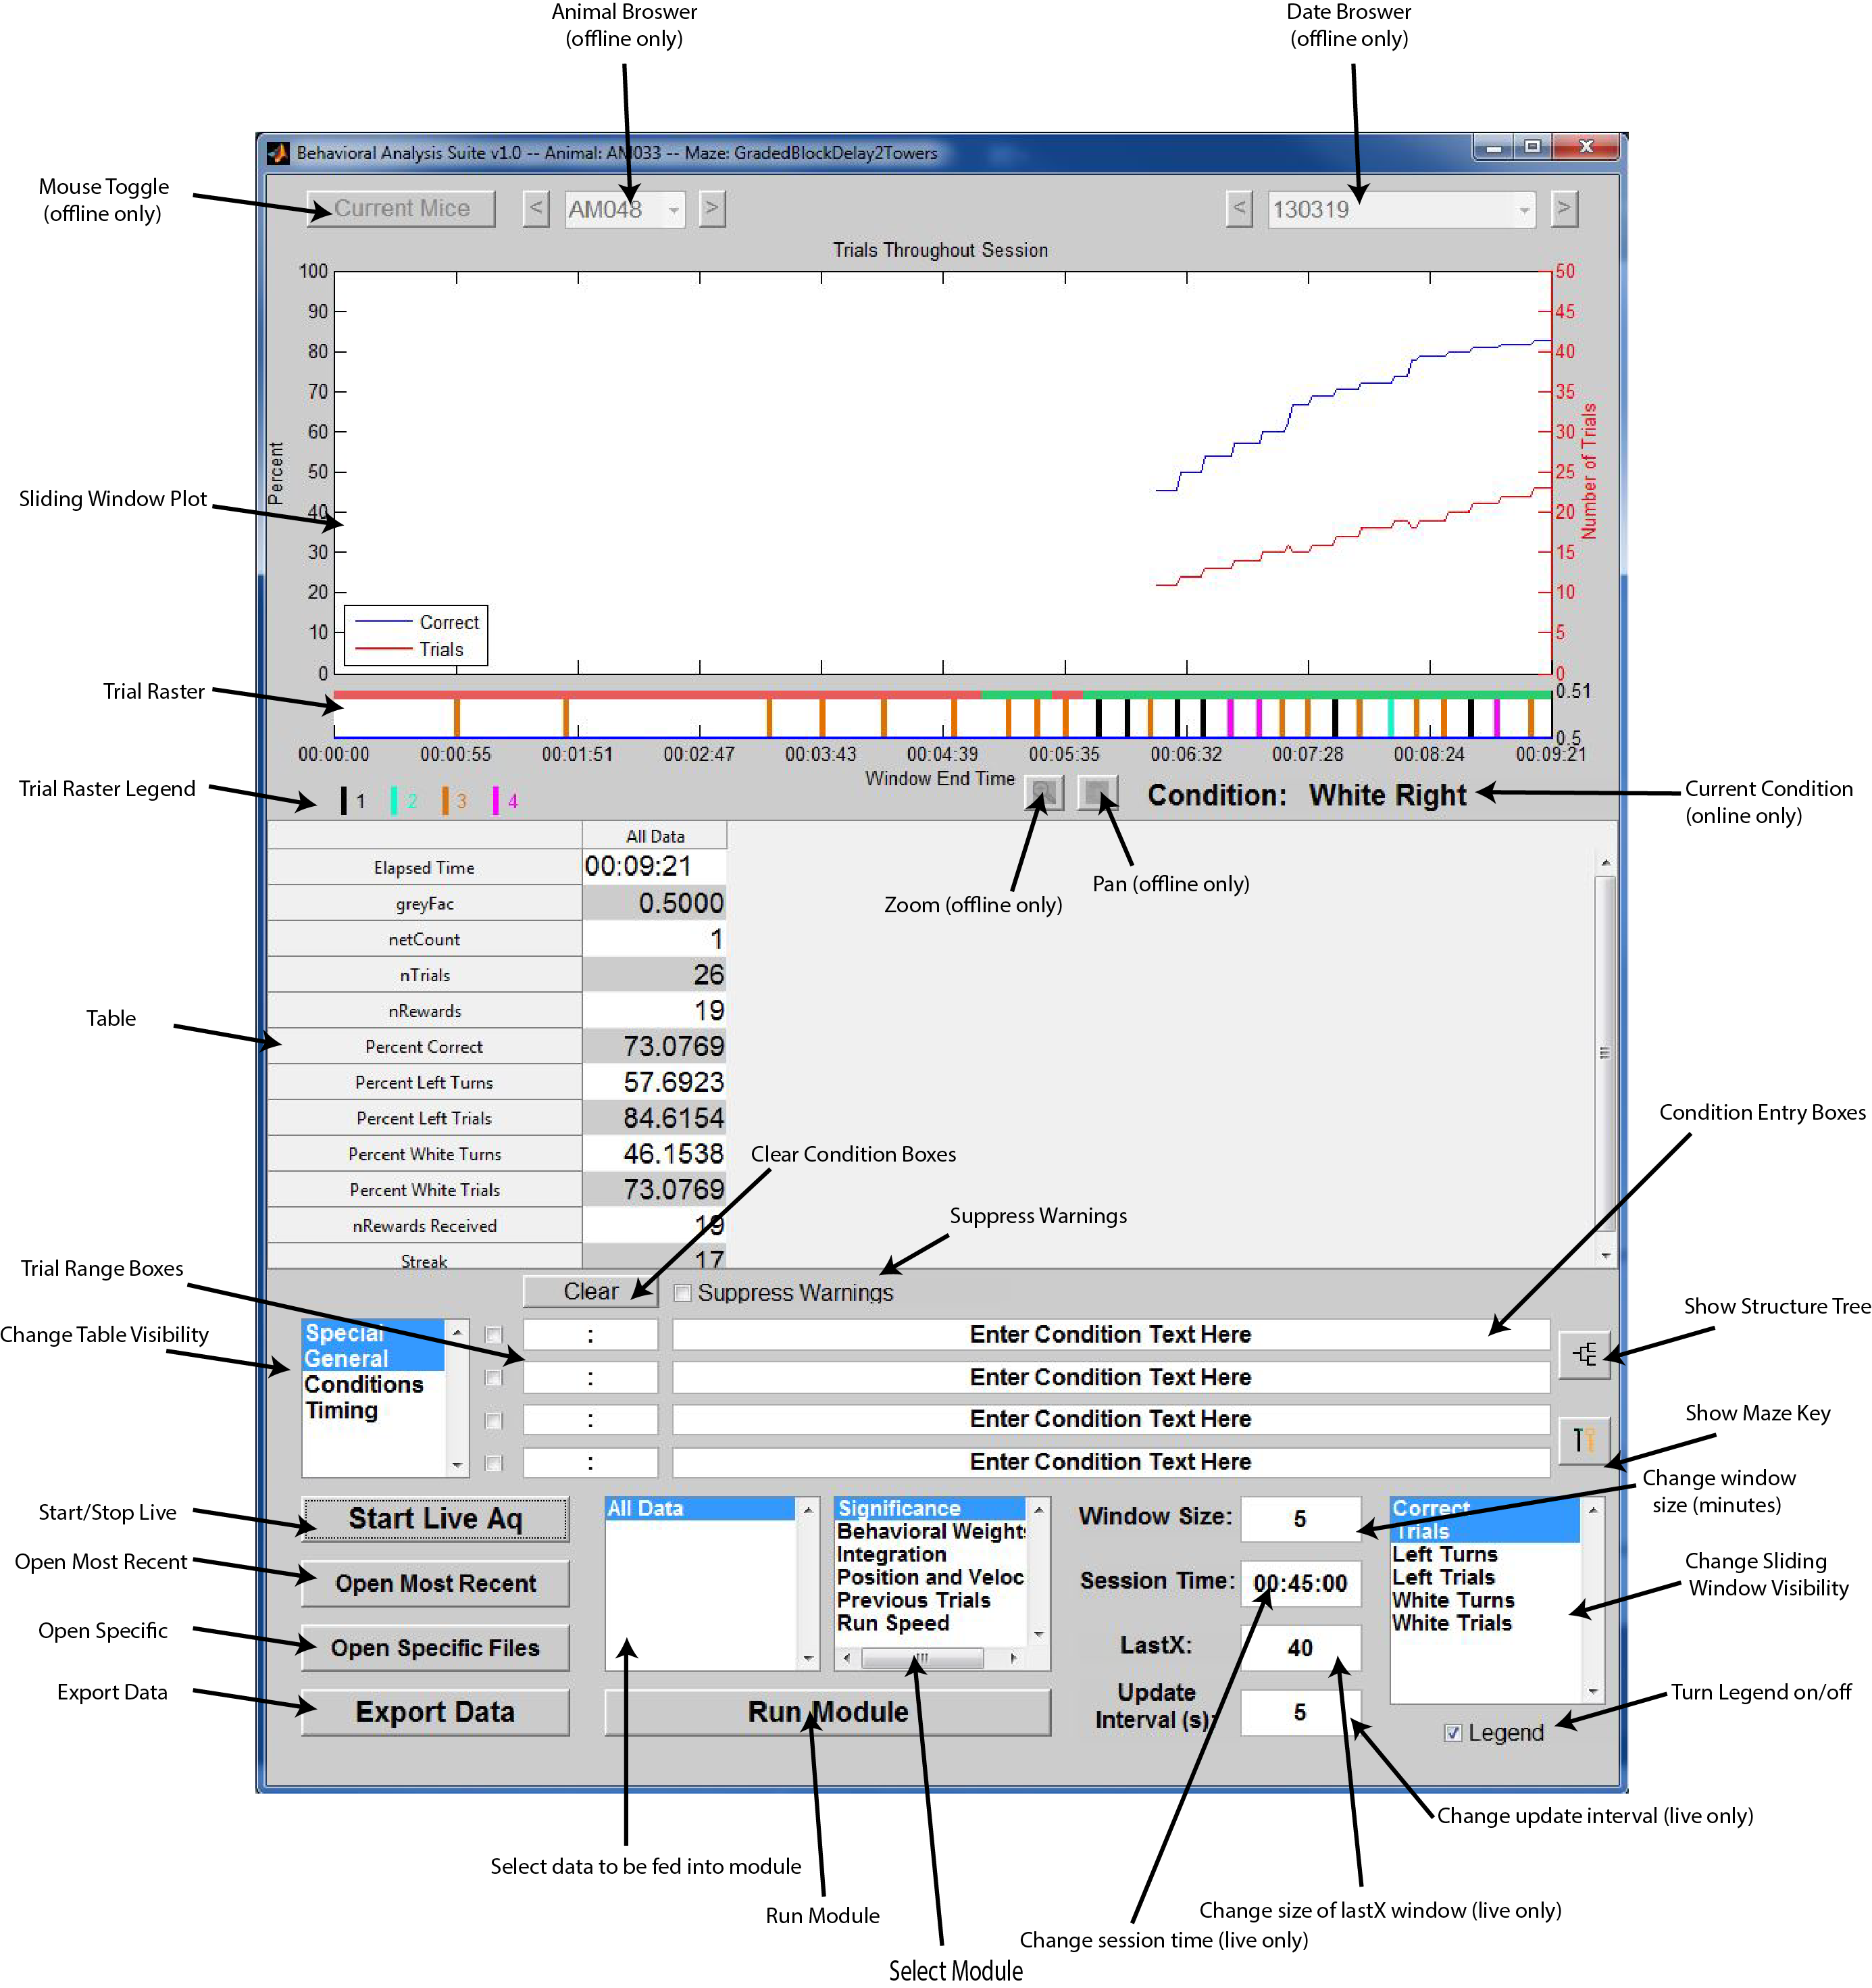
\includegraphics[width=0.99\textwidth,center]{figures/fig_2_10.png}
\caption[Behavioral analysis suite.]{
\textbf{Behavioral analysis suite.} Graphical interface of the behavioral analysis suite with arrows indicating each component.
\label{fig:2_10}}
\end{figure}

I have also developed the \textit{Behavioral Analysis Suite} (BAS), a MATLAB-based software package for the analysis of behavioral data. The BAS is a modular software package that can be used both graphically and programmatically to analyze any behavioral task with a discrete trial structure\footnote{\noindent The design of data structure underlying the BAS was inspired by discussions with Alex Trott and Alex Wiltschko.}. It has several key features. First, it enables the easy filtering of trials according to any combination of task parameters. For example, in the delayed-match-to-sample task described \hyperref[sec:dms]{above}, one could easily extract all black left trials. One can also subset trials according to substantially more complicated filters, such as all white left trials preceded by a white right trial, lasting longer than seven seconds, and in which the mouse made an error. The ability to rapidly create arbitrary trial subsets was essential during the development of the behaviors described in this chapter. Second, the BAS can be used online to analyze and monitor ongoing behavior as well as offline to analyze past behavior. In offline mode, users can easily combine multiple behavioral sessions, even from different animals. Third, filtered data and generated plots can be exported for further analysis and processing. Finally, custom, user-written modules can be added to the graphical interface to perform arbitrary computations on subsets of the data generated by the BAS. This tool allows users to add modules of their own which perform analyses specific to their use cases. An example of the graphical interface is provided in Figure \ref{fig:2_10}.

\bigskip
The behavioral analysis suite is freely available on GitHub\footnote{\url{https://github.com/arimorcos/BehaviorAnalysisSuite}}.

\section{Thoughts on task design} \label{sec:thoughts_task}

The tasks described in this chapter demonstrate that mice can perform complex decision tasks requiring the extensive use of working memory. However, it also highlights the difficulty of designing, training, and interpreting such tasks. For example, during the \hyperref[sec:dms]{delayed-match-to-sample task}, which is designed to identify neural signals of abstract decision-making that are independent of motor actions, some mice systematically shifted their view angle during the delay period in response to the cue (Figure 2.5g). It is therefore difficult to determine whether the mouse is actually remembering the cue, or merely using its view angle as a form of ‘memory’. This example highlights the difficulty of interpreting the strategy taken by animals to perform tasks. Care must be taken to ensure that the task design does not encourage alternative strategies which are close to as effective as the desired task strategy.

\bigskip
One way to reduce the potential for alternate behavioral strategies is to increase behavioral control. This will also reduce external sources of behavioral variance. For example, new tasks should endeavor to reduce variance in view angle across trial conditions. This could be accomplished in two ways. The view angle could be restricted during portions or the entirety of a trial, enabling perfect control. Alternatively, mice could be encouraged to run with repeatable patterns either by including incentives for running straight, such as extra rewards for trials completed quickly, or by punishment for deviations, such as the addition of friction to the environment, substantially slowing the pace of mice with extreme view angles. However, even with more tightly controlled tasks, we can never eliminate all sources of behavioral variance, so measured caution must always be taken in the interpretation of neural signals.

\bigskip
We should also seek to engineer systems allowing for the rapid prototyping of task designs. This is a critical advantage of the VR system described \hyperref[sec:vr]{above}. Many task designs that may at first seem unlikely to be successful can prove to be highly effective. For example, in training the delayed-match-to-sample task, the 'paired' strategy was essential to induce mice to pay attention to the cue configuration (see Section \ref{sec:dms_train}). This design seemed likely to induce mice to simply repeat choices which led to a reward. However, only a small fraction of mice ever learned this strategy. This example illustrates both the difficulty of predicting how animals will react to certain task designs and highlights the utility of rapid prototyping. If the cost of attempting such a strategy had been high, we likely never would have attempted it. 

\bigskip
Because tasks can vary dramatically in the amount of effort required for their development and training, we should also seek to use the simplest task possible for a given scientific question. For example, the delayed-match-to-sample evidence accumulation task proved incredibly difficult to train reliably, while the fixed association evidence accumulation task, in comparison, was trivial to train and develop. However, almost all of the scientific questions answerable by the former task could also be answered by the latter task, with the notable exception of questions seeking to dissociate sensory responses from motor responses. The benefits of a simpler task for the majority of scientific questions may therefore outweigh the cost of reduced interpretability.


